\documentclass[reprint, amsmath, amssymb, aps, pra, nofootinbib]{revtex4-2}

% --- Основные пакеты ---
\usepackage{iftex}
\ifPDFTeX
  \usepackage[T2A]{fontenc}
  \usepackage[utf8]{inputenc}
  \usepackage[russian,english]{babel}
\else
  % при сборке через XeLaTeX/LuaLaTeX: Computer Modern Unicode из папки fonts/
  \usepackage{fontspec}
  \setmainfont{cmunrm}[Path=fonts/, Extension=.otf,
    BoldFont=cmunbx, ItalicFont=cmunti, BoldItalicFont=cmunbi]
  \setmonofont{cmuntt}[Path=fonts/, Extension=.otf]
  \usepackage{polyglossia}
  \setdefaultlanguage{russian}
  \setotherlanguage{english}
\fi

\usepackage{graphicx}
\graphicspath{{figures/}}
\usepackage{bm}

\usepackage[unicode, colorlinks=true, linkcolor=blue, citecolor=blue, urlcolor=blue]{hyperref}

\begin{document}

\title{3.5.2 Изучение плазмы индукционного газового разряда}

\author{Иван Рудко}
\email{rudko.ia@phystech.edu}
\affiliation{Московский физико-технический университет, группа Б02-506}

\author{Ефим Сычев}
\email{sychev.ea@phystech.edu}
\affiliation{Московский физико-технический университет, группа Б02-506}

\date{\today}
\begin{abstract}
Методом двойного зонда исследована плазма высокочастотного индукционного разряда в воздухе при давлениях от $8\cdot10^{-2}$ до $2\cdot10^{-1}$~торр. Зондовые вольт-амперные характеристики сфотографированы с экрана осциллографа, оцифрованы и обработаны с помощью скриптов на Python. По пересечению линейных асимптот с осью ординат и наклону характеристики в нуле найдены ионный ток насыщения и температура электронов, по формуле Бома определена концентрация заряженных частиц. В исследованном диапазоне давлений получено: $k_B T_e \approx 5$--$9$~эВ ($T_e \sim 10^5$~К $\gg T_i$, плазма неравновесная), $n_e \approx (0.9$--$2.1)\cdot10^9$~см$^{-3}$, плазменная частота $\omega_p \approx (1.7$--$2.6)\cdot10^9$~рад/с, электронная поляризационная длина $r_{De} \approx 0.4$--$0.7$~мм, дебаевский радиус экранирования $r_D \approx 26$--$39$~мкм, число ионов в дебаевской сфере $N_D \approx 150$--$230$, степень ионизации $\alpha \approx (1.5$--$7.5)\cdot10^{-7}$. Установлено, что исследуемая плазма является квазинейтральной, идеальной и слабоионизованной.
\end{abstract}

\maketitle

% --- Основной текст ---
\section{Введение}
При достаточно высокой степени ионизации газа кулоновское взаимодействие заряженных частиц приводит к их коллективному движению, и среда проявляет качественно новые свойства по сравнению с нейтральным газом. Такое состояние вещества называют плазмой~\cite{practicum2019}. К её основным свойствам относятся высокая электропроводность и квазинейтральность: подвижные заряды распределяются в пространстве так, что средняя плотность заряда обращается в нуль, а разделение зарядов возникает лишь на микроскопических масштабах вследствие тепловых флуктуаций.

Из-за непрерывной рекомбинации электронов и ионов стационарное состояние плазмы поддерживается только за счёт внешнего источника энергии, в частности электрического разряда в газе. В исследуемой установке разряд возбуждается переменным радиочастотным полем в стеклянной трубке с разреженным воздухом, помещённой внутрь катушки индуктивности колебательного контура. Высокочастотный ток в соленоиде индуцирует вихревое электрическое поле, силовые линии которого, как и линии разрядного тока, замкнуты в окружности; такой безэлектродный разряд называют кольцевым, индукционным или разрядом $H$-типа.

В низкотемпературной газоразрядной плазме ионизована лишь малая доля молекул, а сама система существенно неравновесна ($T_e \gg T_i$). Из-за большой разницы масс ($m_e \ll m_i$) обмен энергией при упругих столкновениях электронов с тяжёлыми частицами затруднён: электроны эффективно разогреваются вихревым полем до температур $T_e \sim 10^4$--$10^5$~К, тогда как ионы быстро передают кинетическую энергию нейтральным молекулам газа и стенкам камеры, оставаясь при температуре вблизи комнатной ($T_i \sim 300$~К). В работе свойства плазмы индукционного разряда при различных давлениях воздуха исследовались методом двойного зонда: путём автоматизированной аппроксимации вольт-амперных характеристик в Python определялись температура и концентрация электронов, по которым рассчитывались плазменная частота, дебаевские длины, число частиц в дебаевской сфере и степень ионизации газа.

\section{Физические основы явления}
Здесь и далее, как принято в физике плазмы, все соотношения записаны в гауссовой системе единиц (СГС).

\subsection{Основные характеристики плазмы}
При смещении электронов в некотором объёме квазинейтральной плазмы ($n_e = n_i$) относительно малоподвижных ионов на малое расстояние $\Delta x$ на границах области возникают нескомпенсированные поверхностные заряды. Создаваемое ими однородное поле $E = 4\pi n_e e \Delta x$ действует на электроны как возвращающая сила ($m_e \Delta\ddot{x} = -eE$), что приводит к гармоническим колебаниям электронной компоненты с \textit{плазменной} (ленгмюровской) частотой
\begin{equation}
\omega_p = \sqrt{\frac{4\pi n_e e^2}{m_e}}. \label{eq:omega_p}
\end{equation}
Характерная амплитуда таких колебаний, возбуждаемых тепловым движением, определяется смещением электронов со средней тепловой скоростью $\bar v_e \sim \sqrt{k_B T_e/m_e}$ за время $1/\omega_p$. Эта величина называется дебаевским радиусом и задаёт пространственный масштаб, на котором возможно спонтанное нарушение квазинейтральности. Тот же масштаб определяет эффект плазменного экранирования: пробный заряд $q$, помещённый в плазму, окружается облаком частиц противоположного знака, вследствие чего потенциал поля спадает с расстоянием по закону $\varphi(r) = (q/r)\exp(-r/r_D)$.

В неравновесной плазме ($T_e \neq T_i$) вводятся электронная и ионная дебаевские длины:
\begin{equation}
r_{De} = \sqrt{\frac{k_B T_e}{4\pi n_e e^2}}, \qquad r_{Di} = \sqrt{\frac{k_B T_i}{4\pi n_i e^2}}, \label{eq:r_De_Di}
\end{equation}
а результирующий радиус экранирования поля стороннего заряда определяется выражением
\begin{equation}
r_D = \left(r_{De}^{-2} + r_{Di}^{-2}\right)^{-1/2}. \label{eq:r_D}
\end{equation}
В условиях газового разряда ($T_e \gg T_i$) выполняется соотношение $r_D \approx r_{Di}$, то есть экранирование статического потенциала определяется холодными ионами. Масштаб же тепловых флуктуаций плотности заряда задаётся величиной $r_{De}$, называемой электронной поляризационной длиной.

Ионизованный газ является плазмой, если дебаевский радиус много меньше характерного размера занимаемой области: $r_D \ll a$. Отношение тепловой энергии частиц к энергии их кулоновского взаимодействия по порядку величины совпадает с числом заряженных частиц в сфере радиуса $r_D$:
\begin{equation}
N_D = \frac{4}{3}\pi n_i r_D^3. \label{eq:N_D}
\end{equation}
При $N_D \gg 1$ кулоновское взаимодействие мало по сравнению с тепловой энергией, и плазма считается идеальной.

Диэлектрическая проницаемость плазмы без учёта столкновений в переменном поле частоты $\omega$ равна
\begin{equation}
\varepsilon = 1 - \frac{\omega_p^2}{\omega^2}, \label{eq:epsilon}
\end{equation}
поэтому при $\omega < \omega_p$ величина $\varepsilon$ отрицательна, и электромагнитные волны не могут распространяться в плазме, полностью отражаясь от неё.

\subsection{Зондовый метод}
Проводник, внесённый в плазму, подвергается соударениям с электронами и ионами, плотность потока которых равна $j = \frac{1}{4}n\bar{v}$. Поскольку тепловая скорость электронов $\bar{v}_e = \sqrt{8k_B T_e/\pi m_e}$ значительно превосходит скорость тяжёлых ионов, изолированный проводник заряжается отрицательно относительно плазмы до \textit{плавающего потенциала} $U_f$, при котором электронный и ионный токи на зонд сравниваются:
\begin{equation}
U_f = -\frac{1}{2}\,\frac{k_B T_e}{e}\,\ln\frac{T_e m_i}{T_i m_e}. \label{eq:U_f}
\end{equation}
Вокруг зонда формируется экранирующий дебаевский слой положительного пространственного заряда толщиной порядка $r_D$. Ионы, влетающие в этот слой, ускоряются полем зонда до скоростей $v_i \sim \sqrt{k_B T_e/m_i}$, определяемых температурой горячих электронов. Для расчёта ионного тока насыщения используется полуэмпирическая формула Бома:
\begin{equation}
I_{i\text{н}} \approx 0.4\, n_i e S \sqrt{\frac{2k_B T_e}{m_i}}, \label{eq:Bohm}
\end{equation}
где $S$ --- площадь собирающей поверхности зонда. Вследствие расширения собирающего слоя и ускорения частиц приложенным полем ток насыщения не остаётся строго постоянным и медленно возрастает с увеличением $|U|$.

\subsection{Двойной зонд}
Система двойного зонда состоит из двух идентичных близко расположенных электродов, между которыми создаётся разность потенциалов $U$, малая по сравнению с $|U_f|$. Оба зонда находятся под отрицательным потенциалом вблизи плавающего, то есть работают на ионной ветви характеристики. Ионные токи на оба электрода равны $I_{i\text{н}}$ и взаимно компенсируются в замкнутой цепи, а результирующий ток обусловлен разностью электронных токов, зависящих от потенциала по закону Больцмана:
\begin{equation}
I_{1,2} = I_{i\text{н}}\left[1 - \exp\left(\frac{e\Delta U_{1,2}}{k_B T_e}\right)\right], \label{eq:I_12}
\end{equation}
где $\Delta U_{1,2}$ --- смещения потенциалов зондов относительно $U_f$, причём $U = \Delta U_2 - \Delta U_1$. Поскольку зонды соединены через плазму последовательно ($I_1 = -I_2 = I$), исключение $\Delta U_{1,2}$ из~\eqref{eq:I_12} приводит к уравнению вольт-амперной характеристики (ВАХ) двойного зонда:
\begin{equation}
I = I_{i\text{н}}\,\mathrm{th}\,\frac{eU}{2k_B T_e}. \label{eq:double_probe}
\end{equation}

Реальная ВАХ отличается от идеальной зависимости~\eqref{eq:double_probe} наличием наклона асимптот при больших $|U|$ (рис.~\ref{fig:theory_vah}). При обработке характеристики ионный ток насыщения $I_{i\text{н}}$ определяется по пересечению линейных асимптот с осью ординат ($U = 0$), а электронная температура --- по наклону кривой в начале координат. Дифференцирование~\eqref{eq:double_probe} в точке $U = 0$ даёт
\begin{equation}
k_B T_e = \frac{1}{2}\,\frac{eI_{i\text{н}}}{\left.\dfrac{dI}{dU}\right|_{U=0}}. \label{eq:kT_e}
\end{equation}
Геометрически величина $2k_B T_e/e$ соответствует проекции на ось напряжений отрезка касательной в нуле от начала координат до пересечения с горизонтальной линией $I = I_{i\text{н}}$. По найденным значениям $T_e$ и $I_{i\text{н}}$ из формулы Бома~\eqref{eq:Bohm} рассчитывается концентрация заряженных частиц $n_i = n_e$.

\begin{figure}[h!]
    \centering
    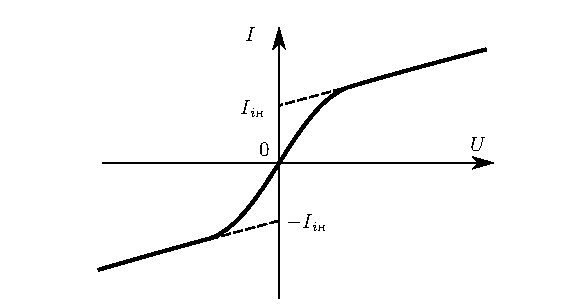
\includegraphics[width=0.8\linewidth]{book_fig5_8.pdf}
    \caption{Ожидаемая вольт-амперная характеристика двойного зонда.}
    \label{fig:theory_vah}
\end{figure}

\subsection{Высокочастотный разряд}
В сильно разреженном газе свободный электрон в гармоническом поле $E = E_0\cos\omega t$ совершает колебания согласно уравнению $m_e \ddot{x} = -eE_0\cos\omega t$, и его средняя за период кинетическая энергия остаётся неизменной. При упругом соударении с тяжёлой молекулой газа ($m_e \ll m_i$) электрон теряет ничтожную долю энергии, но резко изменяет направление импульса. Если после столкновения вектор скорости электрона оказывается сонаправлен с силой со стороны изменившего фазу электрического поля, частица получает от поля дополнительное приращение энергии. В результате серии таких соударений часть электронов разгоняется до энергии ионизации молекул газа даже при относительно малой амплитуде поля, вызывая лавинообразное размножение носителей заряда. Стационарный режим горения разряда устанавливается при динамическом равновесии процессов ударной ионизации и объёмной и пристеночной рекомбинации (наблюдаемое свечение плазмы обусловлено преимущественно рекомбинацией и снятием возбуждения атомов). Установившиеся значения концентрации и температуры электронов определяются родом и давлением газа, а также частотой и мощностью высокочастотного генератора.

\section{Экспериментальная установка}

\begin{figure}[t!]
    \centering
    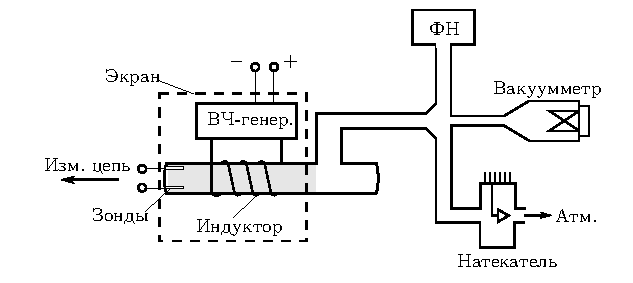
\includegraphics[width=\linewidth]{book_setup.pdf}
    \caption{Схема установки для исследования газового разряда.}
    \label{fig:setup}
\end{figure}

Принципиальная схема вакуумной и газоразрядной частей установки приведена на рис.~\ref{fig:setup}; геометрические параметры камеры и электродов приведены согласно техническому описанию~\cite{manual352}. Разрядная камера представляет собой цилиндрическую стеклянную трубку диаметром 15~мм (радиус $a = 7.5$~мм) и длиной 100~мм, в один из торцов которой впаяны два молибденовых цилиндрических зонда диаметром $d = 0.5$~мм и длиной $l = 10$~мм, расположенные на расстоянии 5~мм друг от друга. Площадь боковой собирающей поверхности каждого зонда без учёта толщины дебаевского слоя составляет $S \approx \pi d l = 15.7$~мм$^2$. Трубка помещена внутрь индуктора --- катушки колебательного контура высокочастотного генератора, работающего на частоте $\sim 10$~МГц. Для защиты измерительной цепи от внешних высокочастотных наводок разрядная камера окружена заземлённым металлическим сетчатым экраном.

Противоположный торец трубки соединён с вакуумной системой. Откачка камеры производится форвакуумным насосом (ФН), а рабочее давление регулируется натекателем, сообщающимся с атмосферой, при непрерывно работающем насосе: в системе устанавливается динамическое равновесие, при котором скорость откачки уравновешивается потоком натекающего воздуха. Проходное сечение натекателя изменяется микрометрическим винтом, воздействующим через пружину на подвижную мембрану клапана, вследствие чего вакуумная система обладает значительной инерционностью. Давление в камере контролируется термопарным вакуумметром ВТ-2 с преобразовательной лампой ЛТ-2 и переводится из показаний шкалы прибора в миллиметры ртутного столба (торры) по градуировочной кривой.

\begin{figure}[t!]
    \centering
    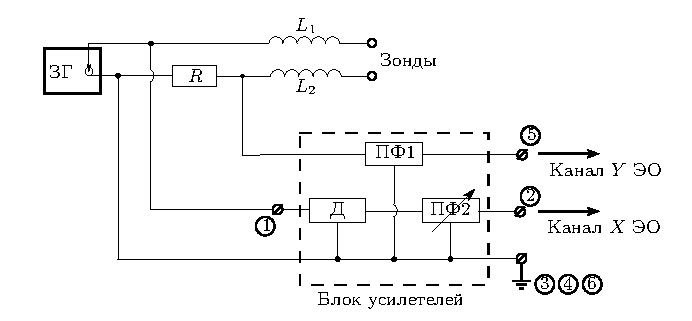
\includegraphics[width=\linewidth]{book_probe_circuit.pdf}
    \caption{Схема измерения зондовых характеристик в разряде.}
    \label{fig:circuit}
\end{figure}

Электрическая схема зондовых измерений показана на рис.~\ref{fig:circuit}. На двойной зонд от генератора звуковой частоты (ЗГ) подаётся синусоидальное напряжение частотой $\approx 50$~Гц. Это же напряжение через делитель Д с коэффициентом деления $1{:}100$ и регулируемый повторитель-фазовращатель ПФ2 поступает на вход горизонтального отклонения (канал $X$) двухканального осциллографа GOS-620. Последовательно с зондами в цепь включён эталонный резистор $R = 100$~кОм; падение напряжения на нём, пропорциональное зондовому току $I$, через нерегулируемый повторитель-фазовращатель ПФ1 подаётся на вход вертикального отклонения (канал $Y$). Включённые последовательно с зондами индуктивности $L_1$ и $L_2$ выполняют роль фильтра нижних частот, блокирующего проникновение сигнала ВЧ-генератора на входы осциллографа. В режиме развёртки $X$--$Y$ на экране наблюдается вольт-амперная характеристика двойного зонда, а фазовый сдвиг между каналами, приводящий к расщеплению кривой в петлю гистерезиса, компенсируется регулировкой фазовращателя ПФ2.

\section{Ход работы}

\subsection{Измерения}

После откачки разрядной камеры форвакуумным насосом и включения ВЧ-генератора по всей длине трубки, включая область расположения зондов, устанавливалось устойчивое свечение разряда. Амплитуда выходного напряжения звукового генератора подбиралась таким образом, чтобы на экране осциллографа регистрировалась вольт-амперная характеристика с выраженными начальными участками насыщения, но без концевых изломов и искажений, возникающих при чрезмерном напряжении вследствие возмущения плазмы полем зондов. Измерения проводились при пяти значениях давления воздуха: $0.08$, $0.09$, $0.10$, $0.15$ и $0.20$~торр. При каждом давлении коэффициенты усиления каналов осциллографа выбирались так, чтобы кривая занимала большую часть экрана, при этом ручки плавной регулировки усиления находились в калиброванном положении. Осциллограммы и чувствительности каналов фотографировались, а показания вакуумметра заносились в протокол.

Пересчёт координат из делений экранной сетки в единицы напряжения и тока с учётом коэффициента деления делителя Д ($1{:}100$) и сопротивления токоизмерительного резистора $R = 100$~кОм осуществляется через масштабные коэффициенты
\begin{equation}
K_U = 100\,k_X, \qquad K_I = \frac{k_Y}{R}, \label{eq:scales}
\end{equation}
где $k_X$ и $k_Y$ --- чувствительности каналов горизонтального и вертикального отклонения (табл.~\ref{tab:scales}). Паспортная инструментальная погрешность коэффициентов отклонения осциллографа GOS-620 составляет $\varepsilon_{k_X} = \varepsilon_{k_Y} = 3\,\%$, относительная погрешность коэффициента деления делителя $\varepsilon_{\text{Д}}$ и сопротивления резистора $\varepsilon_R$ принята равной $1\,\%$, а погрешность определения давления $P$ по градуировочной кривой термопарного вакуумметра ВТ-2 оценена в $\varepsilon_P = 10\,\%$. В соответствии с правилом переноса ошибок для мультипликативных величин относительные инструментальные погрешности масштабных коэффициентов составляют
\begin{equation*}
\varepsilon_{K_U} = \sqrt{\varepsilon_{k_X}^2 + \varepsilon_{\text{Д}}^2} \approx 3.2\,\%, \qquad
\varepsilon_{K_I} = \sqrt{\varepsilon_{k_Y}^2 + \varepsilon_R^2} \approx 3.2\,\%.
\end{equation*}

\begin{table}[h!]
    \caption{Чувствительности каналов осциллографа и масштабные коэффициенты ВАХ.}
    \label{tab:scales}
    \begin{ruledtabular}
        \begin{tabular}{ccccc}
            $P$, торр & $k_X$, В/дел & $k_Y$, В/дел & $K_U$, В/дел & $K_I$, мкА/дел \\
            \colrule
            0.08 & 0.1 & 2.0 & 10 & 20.0 \\
            0.09 & 0.1 & 2.0 & 10 & 20.0 \\
            0.10 & 0.1 & 1.0 & 10 & 10.0 \\
            0.15 & 0.1 & 1.0 & 10 & 10.0 \\
            0.20 & 0.1 & 0.5 & 10 &  5.0 \\
        \end{tabular}
    \end{ruledtabular}
\end{table}

\subsection{Оцифровка осциллограмм}

Для исключения субъективной погрешности ручного переноса кривых на кальку фотографии экрана обрабатывались автоматизированно с помощью скрипта на языке Python с использованием библиотеки компьютерного зрения OpenCV (Прил.~\ref{app:digit}, рис.~\ref{fig:digit_8e2}--\ref{fig:digit_2e1}). На каждом изображении распознавались линии масштабной сетки, и по координатам их узлов строилась матрица проективного преобразования (гомографии) из пикселей в деления шкалы, компенсирующая перспективные искажения и наклон оптической оси камеры; среднеквадратичная невязка привязки узлов сетки не превышала $0.12$~дел. Свечение люминофора выделялось по цветовому порогу, после чего рабочий диапазон по оси $X$ разбивался на вертикальные интервалы шириной $0.1$~дел., внутри каждого из которых вычислялась медианная ордината луча. При наличии нескомпенсированного фазового расщепления усреднённая кривая проходила посередине между ветвями петли, а полуширина интервала между 5-м и 95-м процентилями распределения пикселей принималась за случайную погрешность отсчёта ординаты точки.

При давлении $P = 0.10$~торр (рис.~\ref{fig:digit_1e1}) верхняя ветвь характеристики достигала границы рабочей области экрана, поэтому во избежание искажений, вызванных ограничением сигнала в вертикальном тракте, точки с ординатой $Y > 3.9$~дел. из выборки исключались. При низких давлениях ($0.08$--$0.10$~торр, рис.~\ref{fig:digit_8e2}--\ref{fig:digit_1e1}) на осциллограммах сохранялось незначительное петлеобразное расщепление, которое не удавалось полностью устранить регулировкой фазовращателя ПФ2 вследствие нелинейных фазовых сдвигов в цепи зондов.


\subsection{Температура электронов и ток насыщения}

\begin{figure*}[t!]
    \centering
    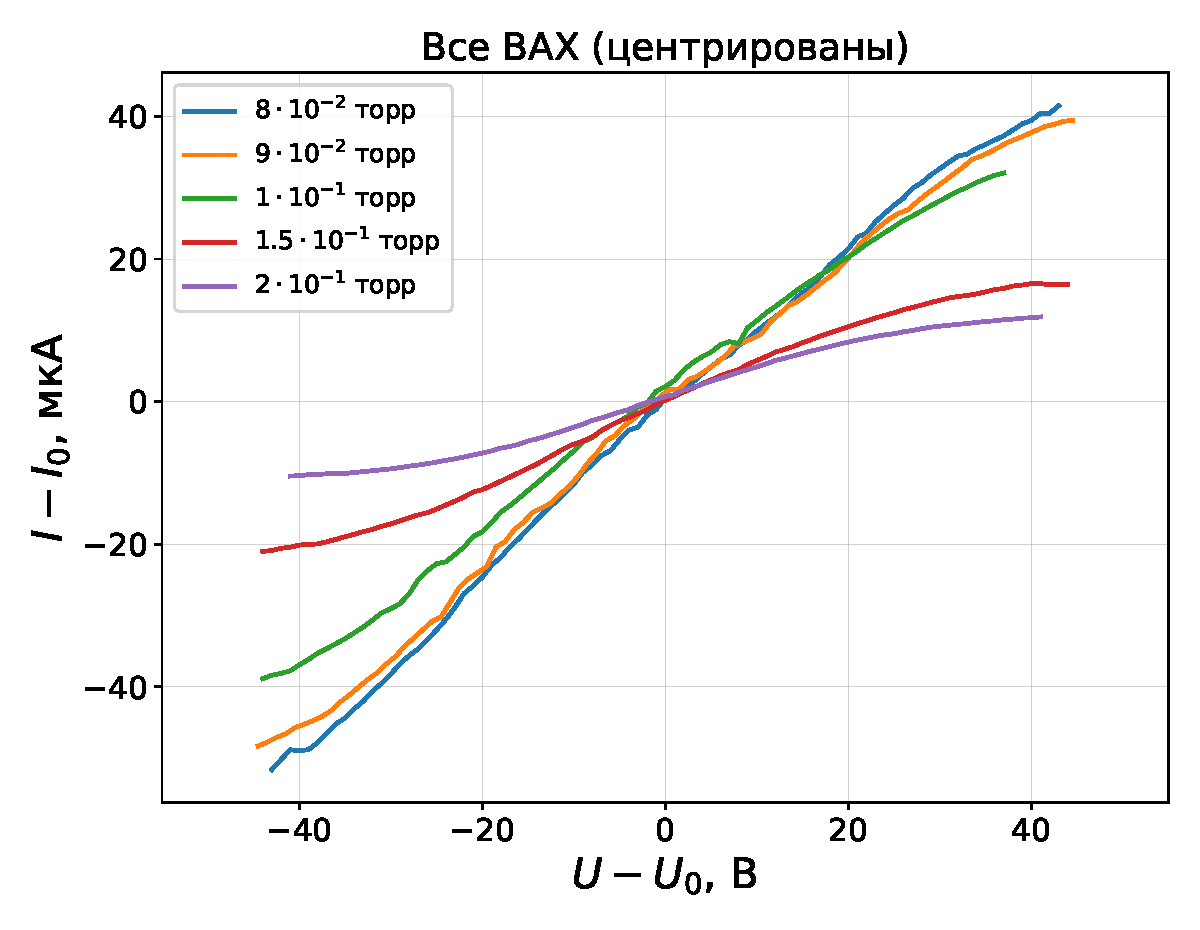
\includegraphics[width=\linewidth]{vah_all.pdf}
    \caption{Семейство вольт-амперных характеристик двойного зонда при различных давлениях воздуха, приведённых к общему началу координат $(U_0, I_0)$.}
    \label{fig:vah}
\end{figure*}

Семейство оцифрованных характеристик в физических координатах $I(U)$, приведённых к единому центру, представлено на рис.~\ref{fig:vah}, а индивидуальные кривые с геометрическими построениями для каждого давления вынесены в Прил.~\ref{app:vah} (рис.~\ref{fig:vah_8e2}--\ref{fig:vah_2e1}). Поскольку положение пучка на экране смещалось регуляторами центровки осциллографа, истинное начало координат характеристики $(U_0, I_0)$ определялось программно из условия симметрии кривой: так как зондирующее напряжение гармоническое и не содержит постоянной составляющей, а зонды идентичны, абсцисса центра $U_0$ полагалась равной середине полного размаха развёртки по напряжению, а ордината $I_0$ находилась как полусумма ординат точек пересечения верхней и нижней асимптот с прямой $U = U_0$.

Параметры ВАХ находились путём линейной аппроксимации методом наименьших квадратов в Python (рис.~\ref{fig:vah_8e2}--\ref{fig:vah_2e1}). Уравнения наклонных асимптот строились по крайним участкам характеристики (по $25\,\%$ размаха напряжения с каждого края), и полуразность их пересечений с осью $U = U_0$ определяла ионный ток насыщения $I_{i\text{н}}$. Дифференциальная проводимость в нуле $s = \left.dI/dU\right|_{U=0}$ находилась из наклона линейной регрессии на центральном участке кривой ($\pm 20\,\%$ от размаха), после чего температура электронов вычислялась по формуле~\eqref{eq:kT_e}.

Для раздельного учёта случайных и инструментальных погрешностей используется метод суперпозиции ошибок в косвенных измерениях. Пусть $\tilde{I}_{i\text{н}}$ (в делениях) и $\tilde{s}$ (в дел./дел.) --- параметры, найденные непосредственно по оцифрованной осциллограмме, так что $I_{i\text{н}} = K_I \tilde{I}_{i\text{н}}$ и $s = (K_I / K_U)\tilde{s}$. Их случайные погрешности $\sigma_{\tilde{I}_{i\text{н}},\text{случ}}$ и $\sigma_{\tilde{s},\text{случ}}$ складываются из дисперсии коэффициентов линейной регрессии и методического разброса, возникающего при варьировании границ интервалов аппроксимации асимптот ($65$--$85\,\%$ размаха) и касательной в нуле ($10$--$30\,\%$ размаха). Полная погрешность ионного тока насыщения определяется квадратичным сложением случайной и приборной составляющих:
\begin{equation}
\sigma_{I_{i\text{н}}} = \sqrt{\left(\frac{\partial I_{i\text{н}}}{\partial \tilde{I}_{i\text{н}}}\sigma_{\tilde{I}_{i\text{н}},\text{случ}}\right)^2 + \left(\frac{\partial I_{i\text{н}}}{\partial K_I}\sigma_{K_I}\right)^2} = I_{i\text{н}}\sqrt{\varepsilon_{\tilde{I}_{i\text{н}},\text{случ}}^2 + \varepsilon_{K_I}^2}. \label{eq:err_Iin}
\end{equation}
При подстановке $I_{i\text{н}}$ и $s$ в выражение~\eqref{eq:kT_e} для электронной температуры вертикальный масштабный коэффициент $K_I$ сокращается: $k_B T_e = e K_U \tilde{I}_{i\text{н}} / (2\tilde{s})$. Дифференцированием этого соотношения по независимым переменным $\tilde{I}_{i\text{н}}$, $\tilde{s}$ и $K_U$ находится относительная погрешность температуры:
\begin{equation}
\varepsilon_{T_e} = \frac{\sigma_{T_e}}{T_e} = \sqrt{\varepsilon_{\tilde{I}_{i\text{н}},\text{случ}}^2 + \varepsilon_{\tilde{s},\text{случ}}^2 + \varepsilon_{K_U}^2}. \label{eq:err_Te}
\end{equation}
Численно перенос погрешностей с учётом корреляции параметров аппроксимации, приборных неопределённостей масштабов и границ участков регрессии выполнялся в Python методом Монте-Карло; в итоговой табл.~\ref{tab:results} приведены медианные значения величин и полуширины доверительного интервала $16$--$84\,\%$ (уровень $1\sigma$).

Во всём исследованном диапазоне давлений получены значения $k_B T_e \approx 5$--$9$~эВ (табл.~\ref{tab:results}). С учётом соотношения $1~\text{эВ} \approx 1.16\cdot10^4$~К это соответствует температуре электронов $T_e \approx (0.6$--$1.1)\cdot10^5$~К; в частности, при $P = 0.20$~торр величина $k_B T_e = 8.3 \pm 0.7$~эВ, откуда $T_e = (9.6 \pm 0.8)\cdot10^4$~К. Найденная температура более чем на два порядка превышает температуру тяжёлых ионов и нейтрального газа ($T_i \approx 300$~К, отношение $T_e/T_i \approx 200$--$370$), что подтверждает сильную термическую неравновесность плазмы ВЧ-разряда. В пределах экспериментальной погрешности зависимость $T_e$ от давления выражена слабо. При давлениях $0.08$--$0.10$~торр (рис.~\ref{fig:vah_8e2}--\ref{fig:vah_1e1}) перегиб характеристик вблизи перехода к насыщению сглажен, и кривые приближаются к линейным, вследствие чего оценка асимптот в этой области менее надёжна.

Помимо учтённых случайных и приборных ошибок, на точность определения $T_e$ влияет систематическая погрешность самой теоретической модели двойного зонда. Во-первых, соотношение~\eqref{eq:double_probe} выведено в предположении малости напряжения между зондами по сравнению с плавающим потенциалом ($|U| \ll |U_f|$). Однако оценка по формуле~\eqref{eq:U_f} для азотной плазмы ($m_i = 28$~а.е.м.) при $k_B T_e \approx 8$~эВ и $T_e/T_i \approx 300$ даёт $|U_f| \approx 70$~В, тогда как амплитуда напряжения развёртки на зондах достигала $\approx 45$~В, что сопоставимо с $|U_f|$. Во-вторых, геометрическая площадь зонда $S = \pi d l$ рассчитывалась в приближении тонкого приэлектродного слоя, тогда как полученная ниже электронная дебаевская длина $r_{De} \approx 0.4$--$0.7$~мм превышает радиус зонда $d/2 = 0.25$~мм, что приводит к увеличению эффективной собирающей поверхности с ростом напряжения. В-третьих, неполное подавление высокочастотных колебаний потенциала плазмы фильтром $L_1, L_2$ вызывает сглаживание ВАХ в окрестности нуля и систематическое завышение измеряемой температуры $T_e$. Вследствие указанных факторов абсолютная точность определения $T_e$ методом двойного зонда составляет по порядку величины десятки процентов, тогда как концентрация $n_e \propto T_e^{-1/2}$ менее чувствительна к систематическому сдвигу температуры.


\subsection{Концентрация, плазменная частота и дебаевские длины}

\begin{figure*}[t!]
    \centering
    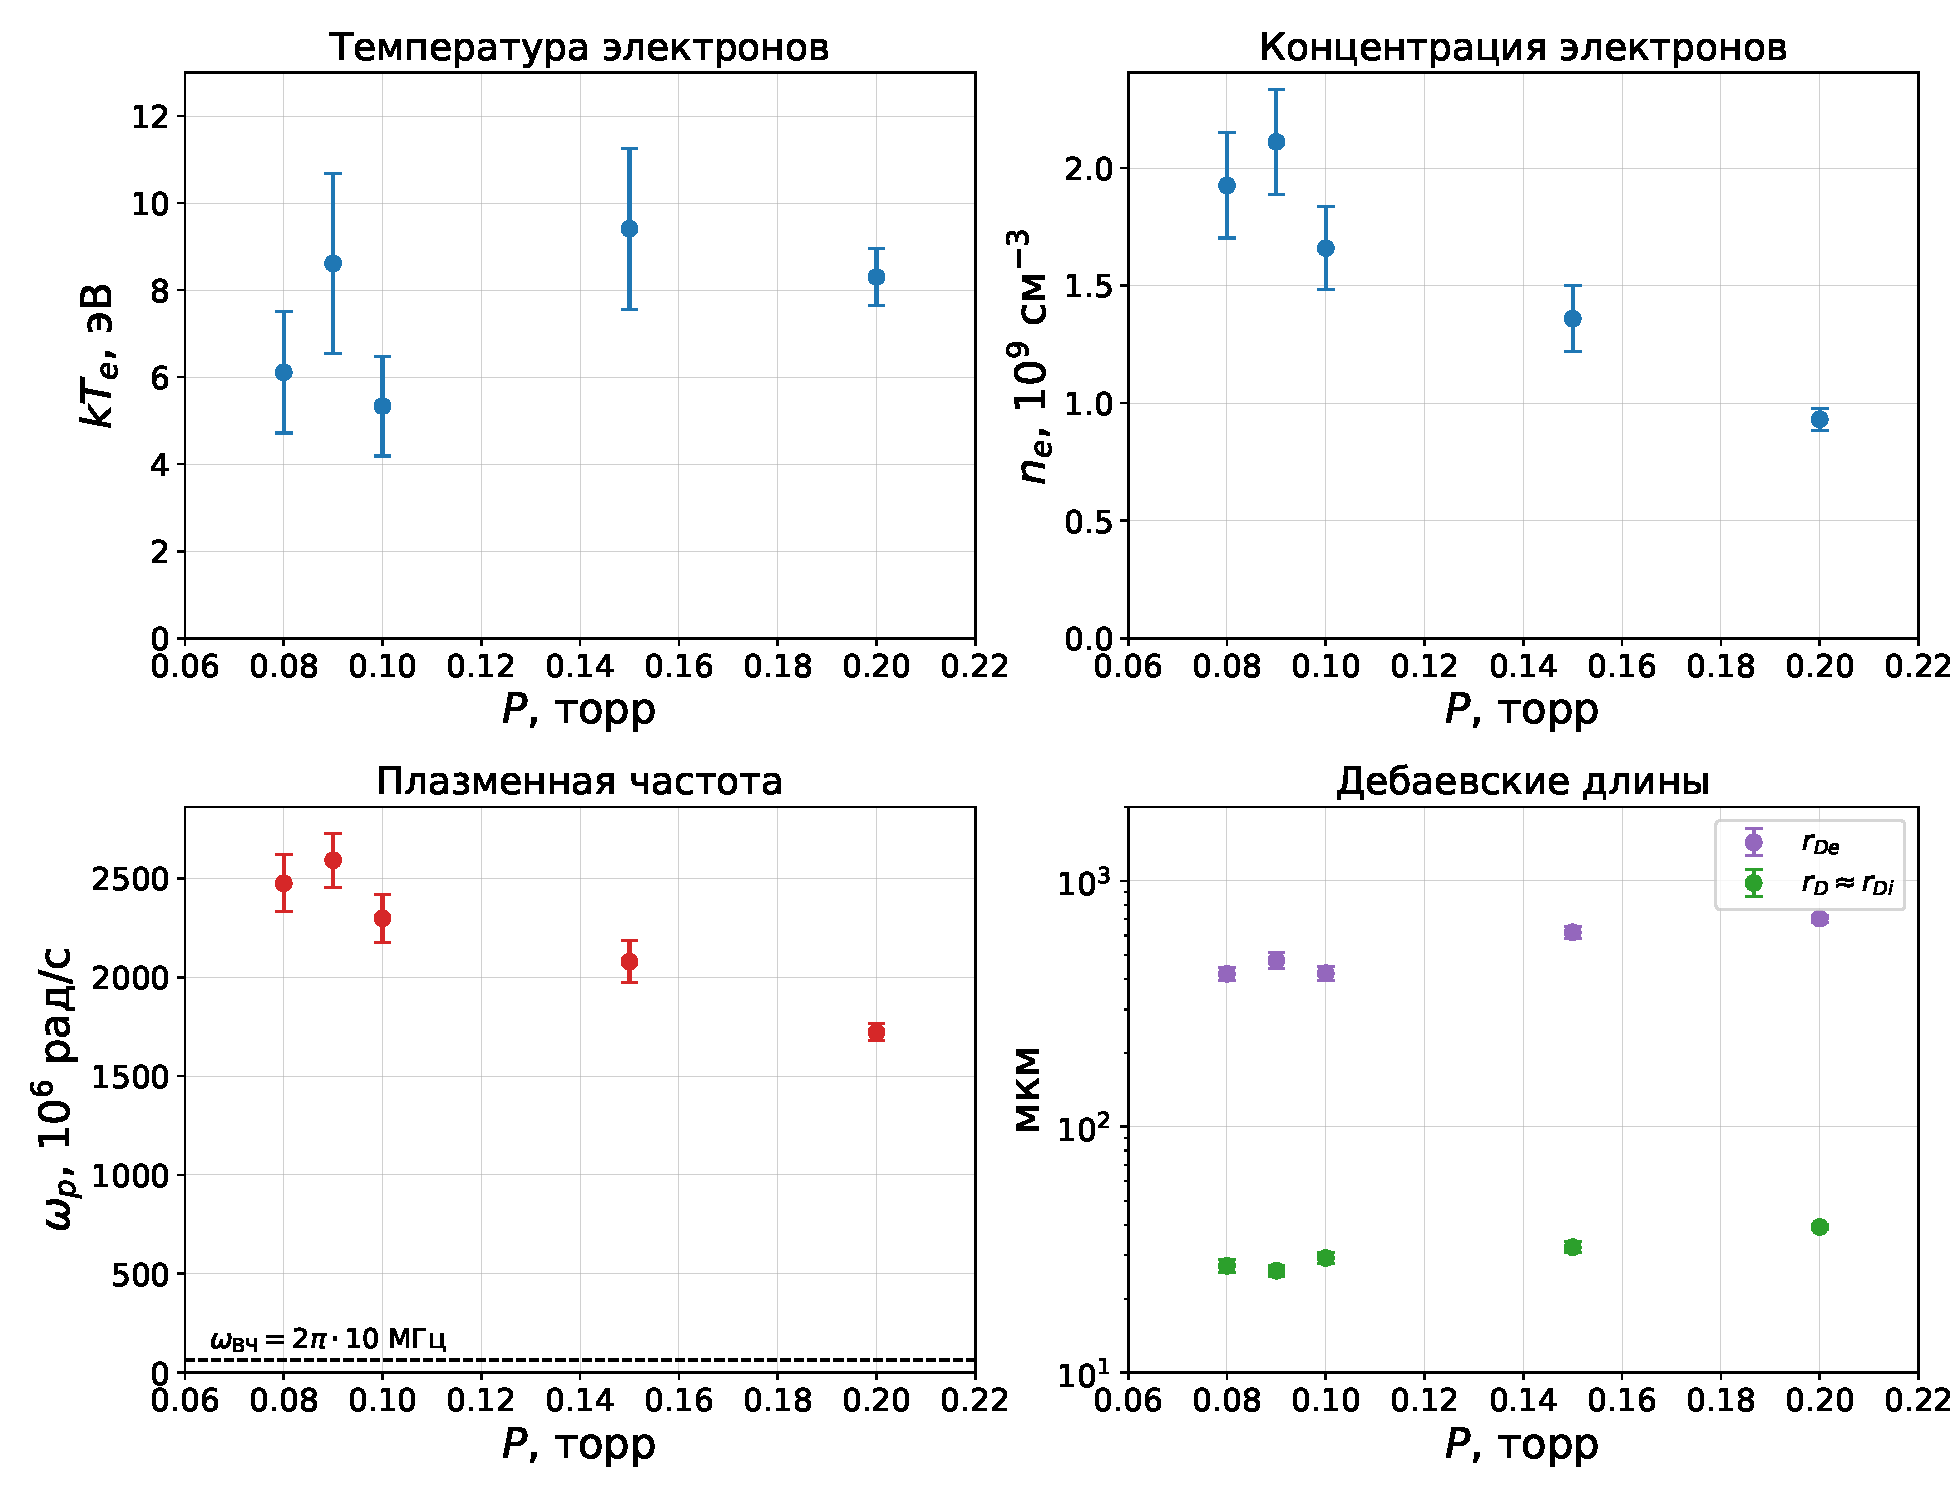
\includegraphics[width=\linewidth]{plasma_vs_p.pdf}
    \caption{Зависимости расчётных параметров плазмы от давления воздуха в разрядной камере. На графике для $\omega_p$ горизонтальной штриховой линией отмечена круговая частота поля ВЧ-генератора ($\omega_{\text{ВЧ}} \approx 6.3\cdot10^7$~рад/с).}
    \label{fig:params}
\end{figure*}

Концентрация заряженных частиц в предположении однократной ионизации ($n_e = n_i$) рассчитывалась по формуле Бома~\eqref{eq:Bohm}:
\begin{equation}
n_e = \frac{I_{i\text{н}}}{0.4\, e S}\sqrt{\frac{m_i}{2k_B T_e}}. \label{eq:ne_calc}
\end{equation}
Поскольку рабочим газом являлся воздух, в расчётах использовалась масса молекулярного иона азота $\text{N}_2^+$ ($m_i = 28$~а.е.м. $= 4.65\cdot10^{-23}$~г; учёт присутствия ионов $\text{O}_2^+$ с массой $32$~а.е.м. увеличивает оценку $n_e$ менее чем на $3\,\%$). Полученные значения концентрации лежат в диапазоне $n_e \approx (0.9$--$2.1)\cdot10^9$~см$^{-3}$ и монотонно убывают с ростом давления (рис.~\ref{fig:params}). Такое поведение объясняется уменьшением длины свободного пробега электронов $\lambda_e \propto 1/P$ при повышении плотности газа: за время между столкновениями электроны набирают в ВЧ-поле меньшую энергию, что снижает частоту ионизации и смещает баланс ионизации и рекомбинации в сторону меньших концентраций. По порядку величины измеренная концентрация согласуется с характерными значениями для плазмы тлеющего разряда низкого давления ($n_e \sim 10^9$--$10^{10}$~см$^{-3}$~\cite{practicum2019}).

Косвенные погрешности расчётных параметров плазмы определяются из соотношений~\eqref{eq:omega_p}--\eqref{eq:N_D}, \eqref{eq:ne_calc} и выражения для степени ионизации $\alpha = n_i / n_{\text{г}}$ (где $n_{\text{г}} = P / k_B T_i$ --- концентрация нейтральных молекул газа при $T_i = 300$~К) путём логарифмического дифференцирования степенных зависимостей:
\begin{equation}
\begin{aligned}
\varepsilon_{n_e} &= \sqrt{\varepsilon_{I_{i\text{н}}}^2 + \frac{1}{4}\varepsilon_{T_e}^2}, \qquad
\varepsilon_{\omega_p} = \varepsilon_{r_D} = \varepsilon_{N_D} = \frac{1}{2}\varepsilon_{n_e}, \\
\varepsilon_{r_{De}} &= \frac{1}{2}\sqrt{\varepsilon_{T_e}^2 + \varepsilon_{n_e}^2}, \qquad
\varepsilon_\alpha = \sqrt{\varepsilon_{n_e}^2 + \varepsilon_P^2}.
\end{aligned}
\label{eq:err_indirect}
\end{equation}

Плазменная частота, вычисленная по формуле~\eqref{eq:omega_p}, составляет $\omega_p \approx (1.7$--$2.6)\cdot10^9$~рад/с, что соответствует линейной частоте ленгмюровских колебаний $f_p = \omega_p/2\pi \approx 270$--$410$~МГц. Согласно выражению для диэлектрической проницаемости~\eqref{eq:epsilon}, полученная плазма прозрачна лишь для электромагнитного излучения сверхвысокочастотного диапазона с частотой выше $0.3$--$0.4$~ГГц (длина волны в вакууме $\lambda \lesssim 1$~м). Круговая частота возбуждающего поля ВЧ-генератора $\omega_{\text{ВЧ}} = 2\pi f_{\text{ВЧ}} \approx 6.3\cdot10^7$~рад/с на полтора порядка меньше плазменной частоты ($\omega_{\text{ВЧ}} \ll \omega_p$, рис.~\ref{fig:params}), поэтому в такой среде диэлектрическая проницаемость отрицательна, а вихревое электрическое поле проникает в плазму за счёт скин-эффекта.

Электронная поляризационная длина~\eqref{eq:r_De_Di} в зависимости от давления изменяется в пределах $r_{De} \approx 0.4$--$0.7$~мм, тогда как полный дебаевский радиус экранирования~\eqref{eq:r_D}, определяемый холодными ионами ($T_i = 300$~К), составляет $r_D \approx r_{Di} \approx 26$--$39$~мкм. Поскольку оба характерных масштаба разделения зарядов существенно меньше радиуса разрядной трубки ($r_D \ll r_{De} \ll a = 7.5$~мм), исследуемый ионизованный газ строго удовлетворяет критерию квазинейтральности и является плазмой.

Среднее число ионов в дебаевской сфере, рассчитанное по формуле~\eqref{eq:N_D} с использованием электронной поляризационной длины $r_{De}$, составляет $N_D \approx 150$--$230$. Выполнение сильного неравенства $N_D \gg 1$ означает, что средняя тепловая энергия частиц более чем на два порядка превосходит потенциальную энергию их кулоновского взаимодействия, то есть исследуемая плазма является идеальной. Степень ионизации воздуха $\alpha = n_i k_B T_i / P$ монотонно падает с ростом давления от $7.5\cdot10^{-7}$ при $P = 0.08$~торр до $1.5\cdot10^{-7}$ при $P = 0.20$~торр, что характеризует среду как слабоионизованную плазму. Все численные результаты и их погрешности сведены в табл.~\ref{tab:results} и проиллюстрированы на рис.~\ref{fig:params}.

\begin{table*}[t!]
    \caption{Сводная таблица экспериментальных и расчётных параметров плазмы ВЧ-разряда. Значения $I_{i\text{н}}$ и $k_B T_e$ получены аппроксимацией оцифрованных ВАХ и расчётом по формуле~\eqref{eq:kT_e}; величины $n_e$, $\omega_p$, $r_{De}$, $r_D$, $N_D$ и $\alpha$ вычислены по соотношениям~\eqref{eq:omega_p}--\eqref{eq:N_D} и~\eqref{eq:ne_calc}. Приведены полные погрешности на уровне $1\sigma$.}
    \label{tab:results}
    \begin{ruledtabular}
        \begin{tabular}{ccccccccc}
            $P$, торр & $I_{i\text{н}}$, мкА & $k_B T_e$, эВ & $n_e$, см$^{-3}$ & $\omega_p$, рад/с & $r_{De}$, мкм & $r_D$, мкм & $N_D$ & $\alpha$ \\
            \colrule
            $8\cdot 10^{-2}$ & $12.6\pm2.8$ & $6.1\pm1.4$ & $(1.93\pm0.22)\cdot10^{9}$ & $(2.48\pm0.14)\cdot10^{9}$ & $419\pm26$ & $27.2\pm1.6$ & $162\pm9$ & $(7.5\pm1.2)\cdot10^{-7}$ \\
$9\cdot 10^{-2}$ & $16\pm4$ & $8.6\pm2.1$ & $(2.11\pm0.22)\cdot10^{9}$ & $(2.59\pm0.14)\cdot10^{9}$ & $474\pm35$ & $26.0\pm1.4$ & $155\pm8$ & $(7.3\pm1.1)\cdot10^{-7}$ \\
$1\cdot 10^{-1}$ & $10.1\pm2.1$ & $5.3\pm1.1$ & $(1.66\pm0.18)\cdot10^{9}$ & $(2.30\pm0.12)\cdot10^{9}$ & $421\pm26$ & $29.3\pm1.5$ & $174\pm9$ & $(5.2\pm0.8)\cdot10^{-7}$ \\
$1.5\cdot 10^{-1}$ & $11.0\pm2.2$ & $9.4\pm1.8$ & $(1.36\pm0.14)\cdot10^{9}$ & $(2.08\pm0.11)\cdot10^{9}$ & $618\pm34$ & $32.4\pm1.7$ & $193\pm10$ & $(2.8\pm0.4)\cdot10^{-7}$ \\
$2\cdot 10^{-1}$ & $7.1\pm0.6$ & $8.3\pm0.6$ & $(9.3\pm0.5)\cdot10^{8}$ & $(1.72\pm0.04)\cdot10^{9}$ & $702\pm24$ & $39.1\pm1.0$ & $233\pm6$ & $(1.45\pm0.16)\cdot10^{-7}$ \\

        \end{tabular}
    \end{ruledtabular}
    \raggedright\footnotesize Примечание: указанные доверительные интервалы включают статистическую погрешность аппроксимации (в том числе вариацию границ линейных участков) и инструментальные погрешности приборов. При давлениях $P = 0.08$--$0.10$~торр переход к участкам насыщения выражен слабо, что снижает достоверность линейной экстраполяции асимптот.
\end{table*}


\section{Заключение}
Методом двойного зонда исследованы параметры плазмы высокочастотного индукционного разряда ($H$-типа) в воздухе в диапазоне давлений $0.08$--$0.20$~торр. Зондовые вольт-амперные характеристики, зарегистрированные на экране осциллографа, были оцифрованы с проективной компенсацией перспективных искажений и аппроксимированы с помощью скриптов на Python. По точкам пересечения линейных асимптот ветвей насыщения с осью ординат и наклону характеристик в начале координат определены ионный ток насыщения $I_{i\text{н}}$ и температура электронов $T_e$.

Установлено, что электронная температура составляет $k_B T_e \approx 5$--$9$~эВ ($T_e \approx (0.6$--$1.1)\cdot10^5$~К) и в пределах погрешности слабо зависит от давления газа. Полученные значения более чем на два порядка превосходят температуру тяжёлых ионов и нейтральных молекул ($T_i \approx 300$~К), что свидетельствует о сильной термической неравновесности плазмы. Концентрация заряженных частиц, рассчитанная по формуле Бома, лежит в пределах $n_e \approx (0.9$--$2.1)\cdot10^9$~см$^{-3}$ и монотонно убывает с ростом давления вследствие уменьшения длины свободного пробега электронов, по порядку величины согласуясь с характерными значениями для газоразрядной плазмы низкого давления ($10^9$--$10^{10}$~см$^{-3}$).

Плазменная частота ленгмюровских колебаний составила $\omega_p \approx (1.7$--$2.6)\cdot10^9$~рад/с ($f_p \approx 270$--$410$~МГц): исследуемая среда прозрачна лишь для электромагнитных волн дециметрового и более коротковолнового диапазонов ($\omega > \omega_p$), тогда как вихревое поле ВЧ-генератора ($\omega_{\text{ВЧ}} \approx 6.3\cdot10^7$~рад/с $\ll \omega_p$) экранируется в скин-слое. Электронная поляризационная длина $r_{De} \approx 0.4$--$0.7$~мм и дебаевский радиус экранирования $r_D \approx 26$--$39$~мкм существенно меньше радиуса разрядной трубки ($a = 7.5$~мм), среднее число частиц в дебаевской сфере велико ($N_D \approx 150$--$230 \gg 1$), а степень ионизации газа мала ($\alpha \approx (1.5$--$7.5)\cdot10^{-7} \ll 1$). Таким образом, выполнение теоретических критериев подтверждает, что исследуемая среда представляет собой квазинейтральную, идеальную и слабоионизованную плазму. Основной вклад в погрешность определения параметров при низких давлениях ($0.08$--$0.10$~торр) вносят слабо выраженный переход характеристик к режиму ионного насыщения и остаточный фазовый сдвиг в измерительной цепи, а также систематические погрешности приближения тонкого дебаевского слоя ($r_{De} > d/2$).

% ================= ПРИЛОЖЕНИЯ =================
\appendix

\section{Результаты оцифровки осциллограмм}\label{app:digit}
В данном приложении приведены результаты автоматизированной покадровой обработки фотографий экрана осциллографа для пяти исследованных давлений воздуха ($P = 0.08$, $0.09$, $0.10$, $0.15$ и $0.20$~торр, рис.~\ref{fig:digit_8e2}--\ref{fig:digit_2e1}). На каждом рисунке сопоставлены исходный снимок экрана с наложенной распознанной координатной сеткой (красные линии, жёлтыми выделены центральные оси) и извлечённой средней линией луча (пурпурная кривая), а также результат проективного преобразования выделенных пикселей люминофора в безразмерные координаты делений шкалы экрана с доверительной полосой между 5-м и 95-м процентилями, определяющей суммарную ширину следа луча и раствор остаточной фазовой петли.

\begin{figure*}[t!]
    \centering
    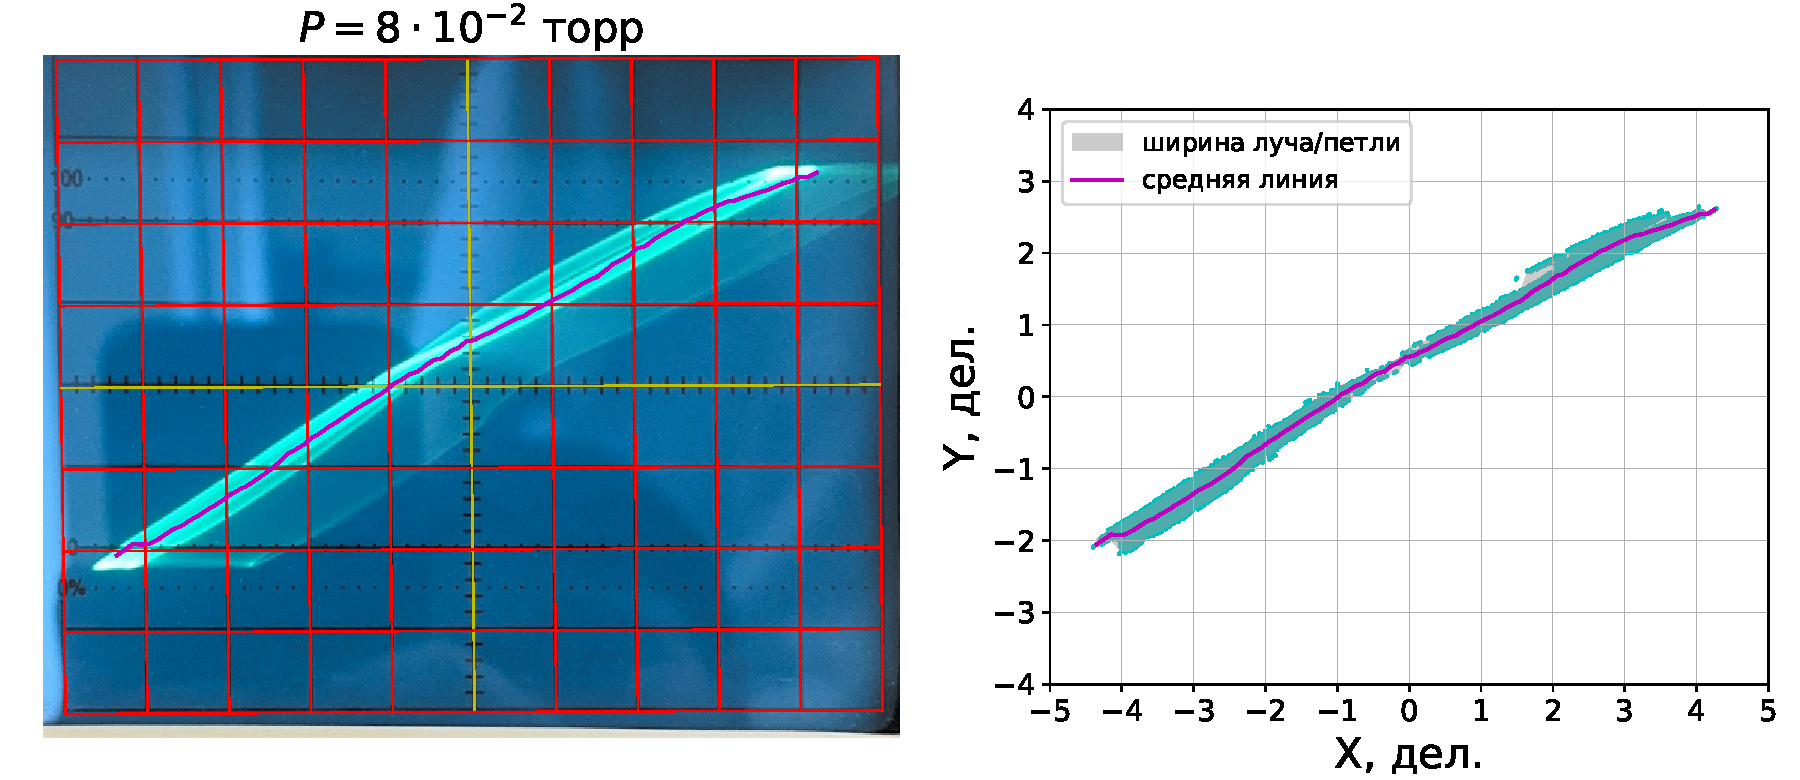
\includegraphics[width=0.8\linewidth]{digitization_check_8e-2.pdf}
    \caption{Верификация распознавания координатной сетки и оцифровки зондовой ВАХ при давлении $P = 0.08$~торр.}
    \label{fig:digit_8e2}
\end{figure*}

\begin{figure*}[t!]
    \centering
    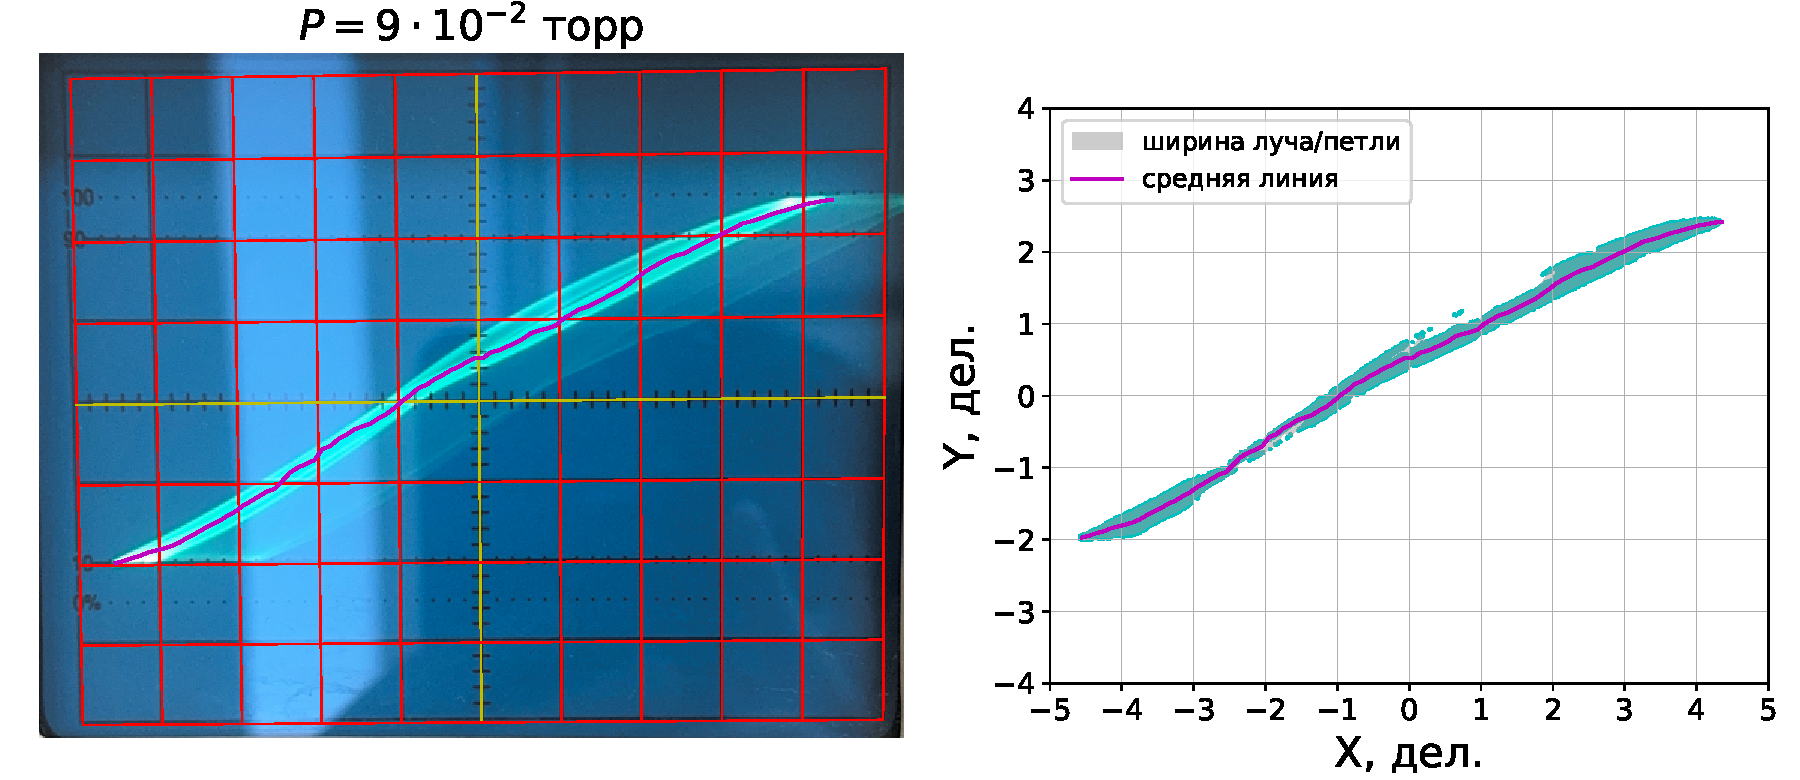
\includegraphics[width=0.8\linewidth]{digitization_check_9e-2.pdf}
    \caption{Верификация распознавания координатной сетки и оцифровки зондовой ВАХ при давлении $P = 0.09$~торр.}
    \label{fig:digit_9e2}
\end{figure*}

\begin{figure*}[t!]
    \centering
    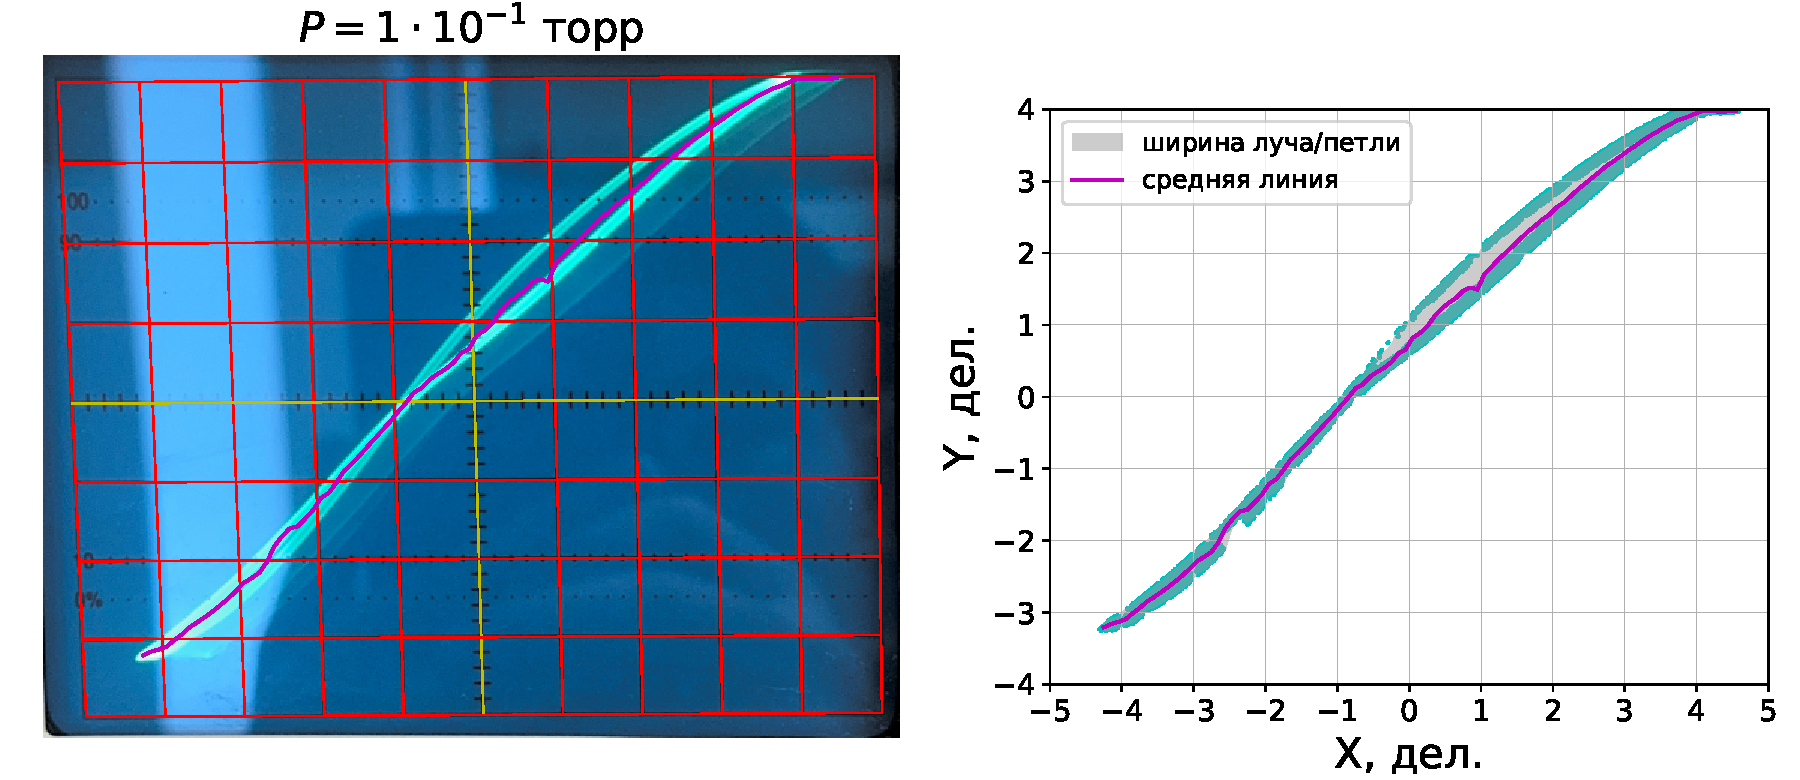
\includegraphics[width=0.8\linewidth]{digitization_check_1e-1.pdf}
    \caption{Верификация распознавания координатной сетки и оцифровки зондовой ВАХ при давлении $P = 0.10$~торр (точки в области насыщения вертикального тракта при $Y > 3.9$~дел. отброшены).}
    \label{fig:digit_1e1}
\end{figure*}

\begin{figure*}[t!]
    \centering
    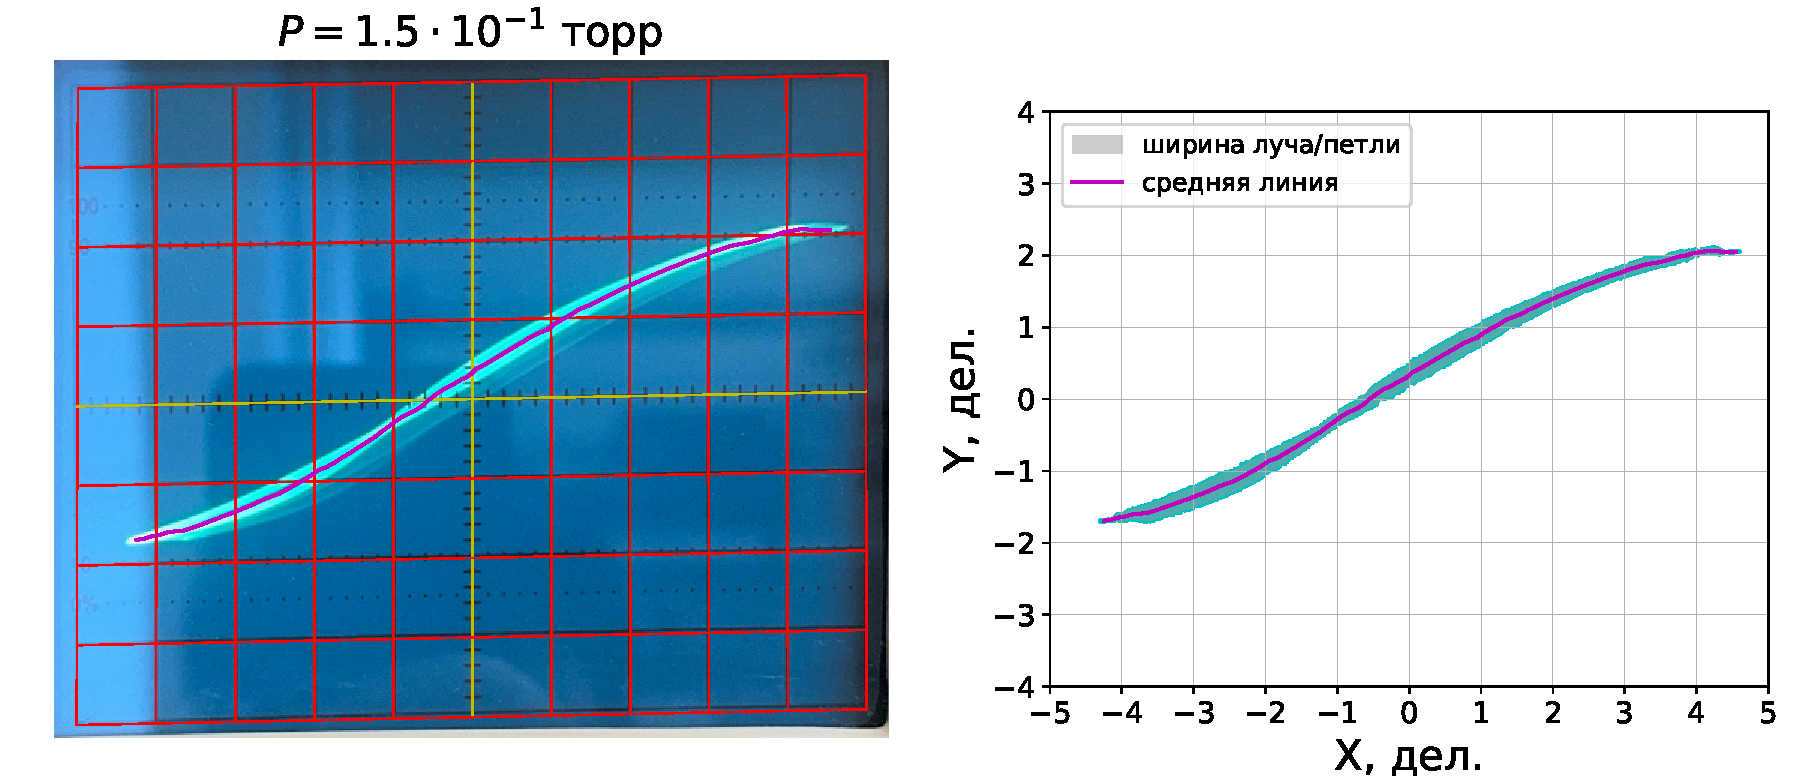
\includegraphics[width=0.8\linewidth]{digitization_check_1.5e-1.pdf}
    \caption{Верификация распознавания координатной сетки и оцифровки зондовой ВАХ при давлении $P = 0.15$~торр.}
    \label{fig:digit_15e1}
\end{figure*}

\begin{figure*}[t!]
    \centering
    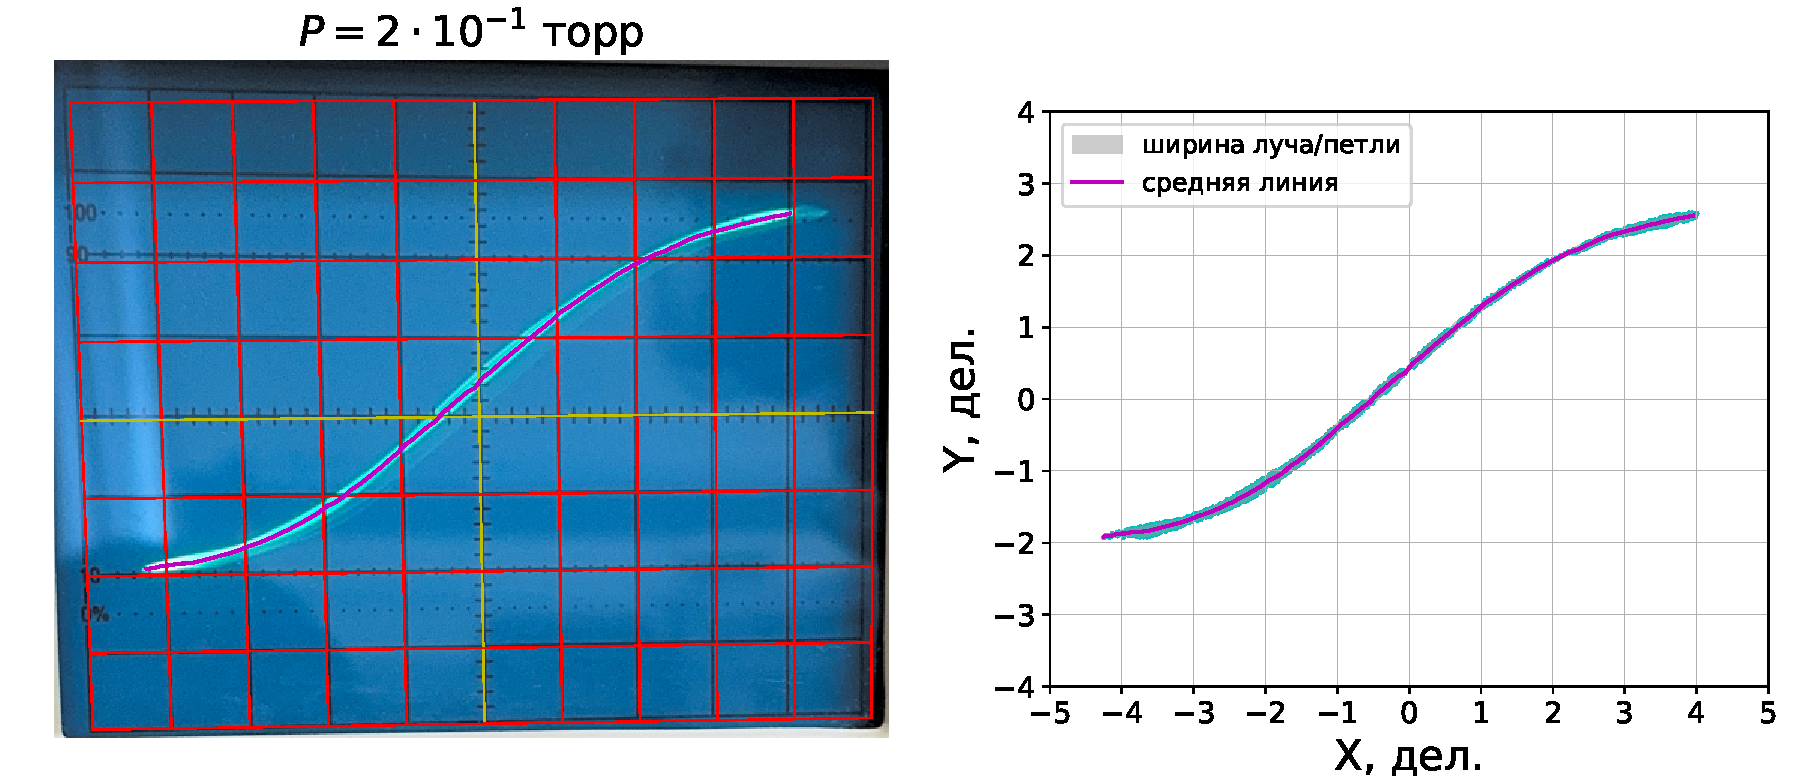
\includegraphics[width=0.8\linewidth]{digitization_check_2e-1.pdf}
    \caption{Верификация распознавания координатной сетки и оцифровки зондовой ВАХ при давлении $P = 0.20$~торр.}
    \label{fig:digit_2e1}
\end{figure*}



\section{Аппроксимация вольт-амперных характеристик двойного зонда}\label{app:vah}
В данном приложении приведены пересчитанные в физические единицы и центрированные вольт-амперные характеристики двойного зонда для пяти исследованных давлений воздуха ($P = 0.08$, $0.09$, $0.10$, $0.15$ и $0.20$~торр, рис.~\ref{fig:vah_8e2}--\ref{fig:vah_2e1}). На каждом графике точками нанесена оцифрованная средняя линия луча, серой областью показана суммарная ширина луча и фазовой петли (интервал между 5-м и 95-м процентилями), зелёными штриховыми прямыми изображены линейные асимптоты ветвей ионного насыщения, чёрной пунктирной прямой --- касательная к характеристике в начале координат, а фиолетовым горизонтальным отрезком отмечена величина $\Delta U = 2k_B T_e/e$.

\begin{figure*}[t!]
    \centering
    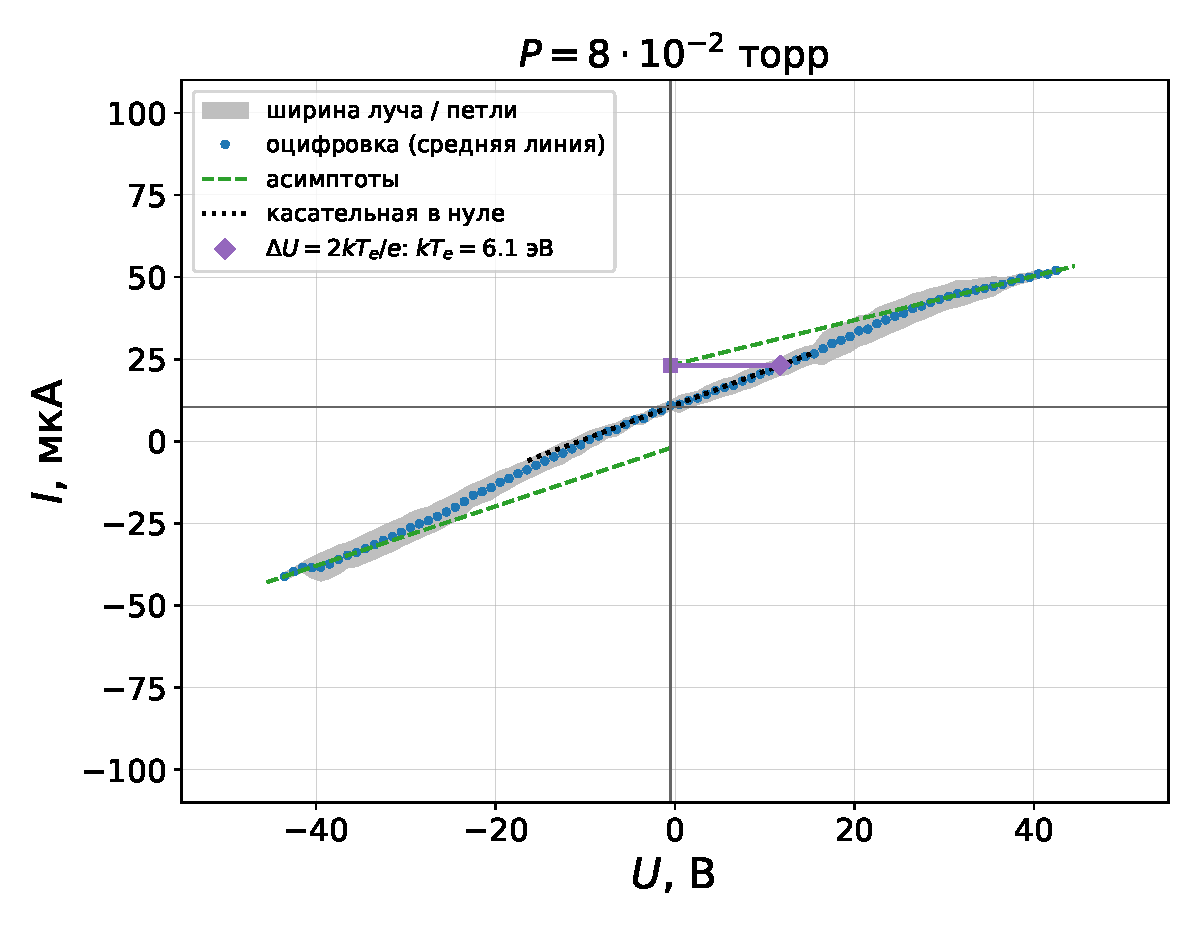
\includegraphics[width=0.8\linewidth]{vah_8e-2.pdf}
    \vspace{-1.5em} \caption{Вольт-амперная характеристика двойного зонда и определение её параметров при давлении $P = 0.08$~торр.}
    \label{fig:vah_8e2}
\end{figure*}

\begin{figure*}[t!]
    \centering
    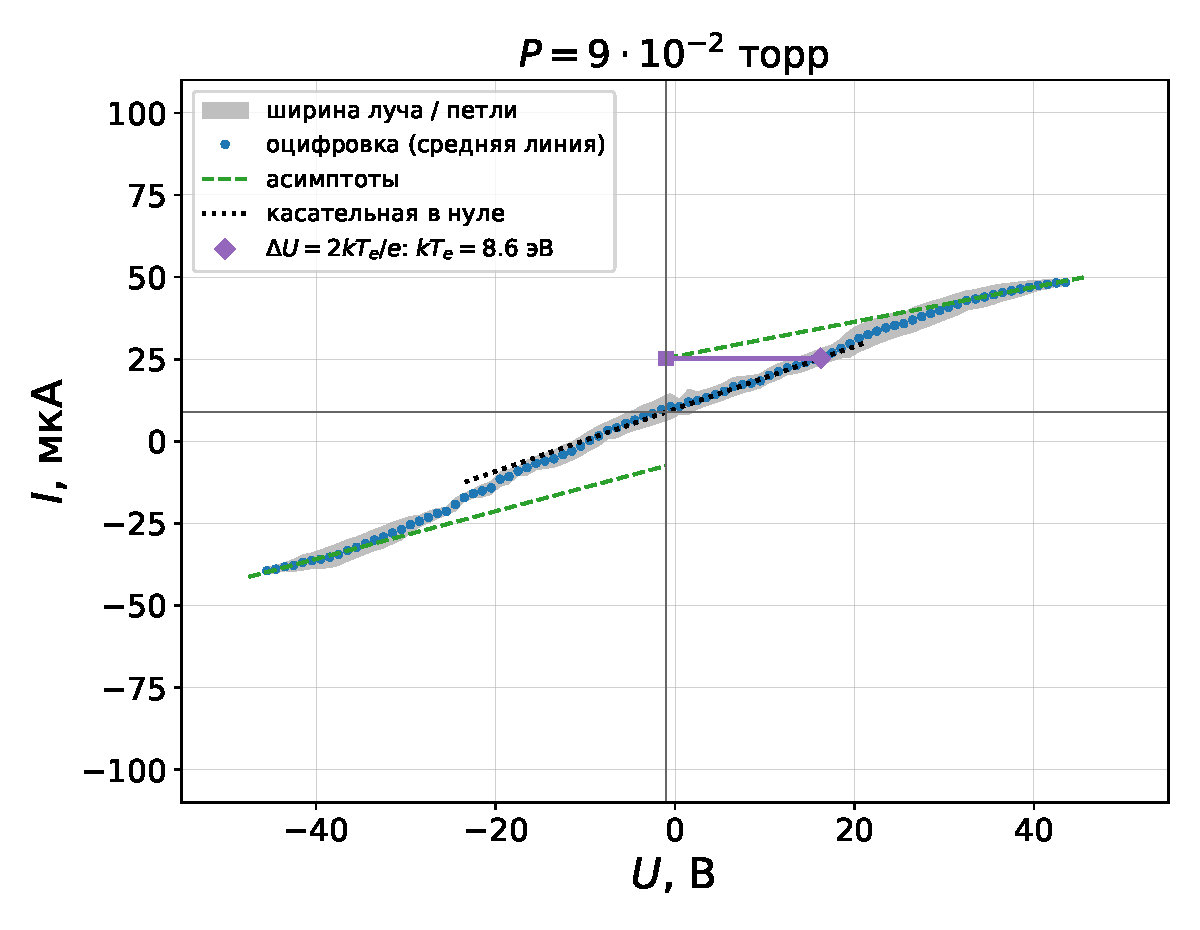
\includegraphics[width=0.8\linewidth]{vah_9e-2.pdf}
    \vspace{-1.5em} \caption{Вольт-амперная характеристика двойного зонда и определение её параметров при давлении $P = 0.09$~торр.}
    \label{fig:vah_9e2}
\end{figure*}

\begin{figure*}[t!]
    \centering
    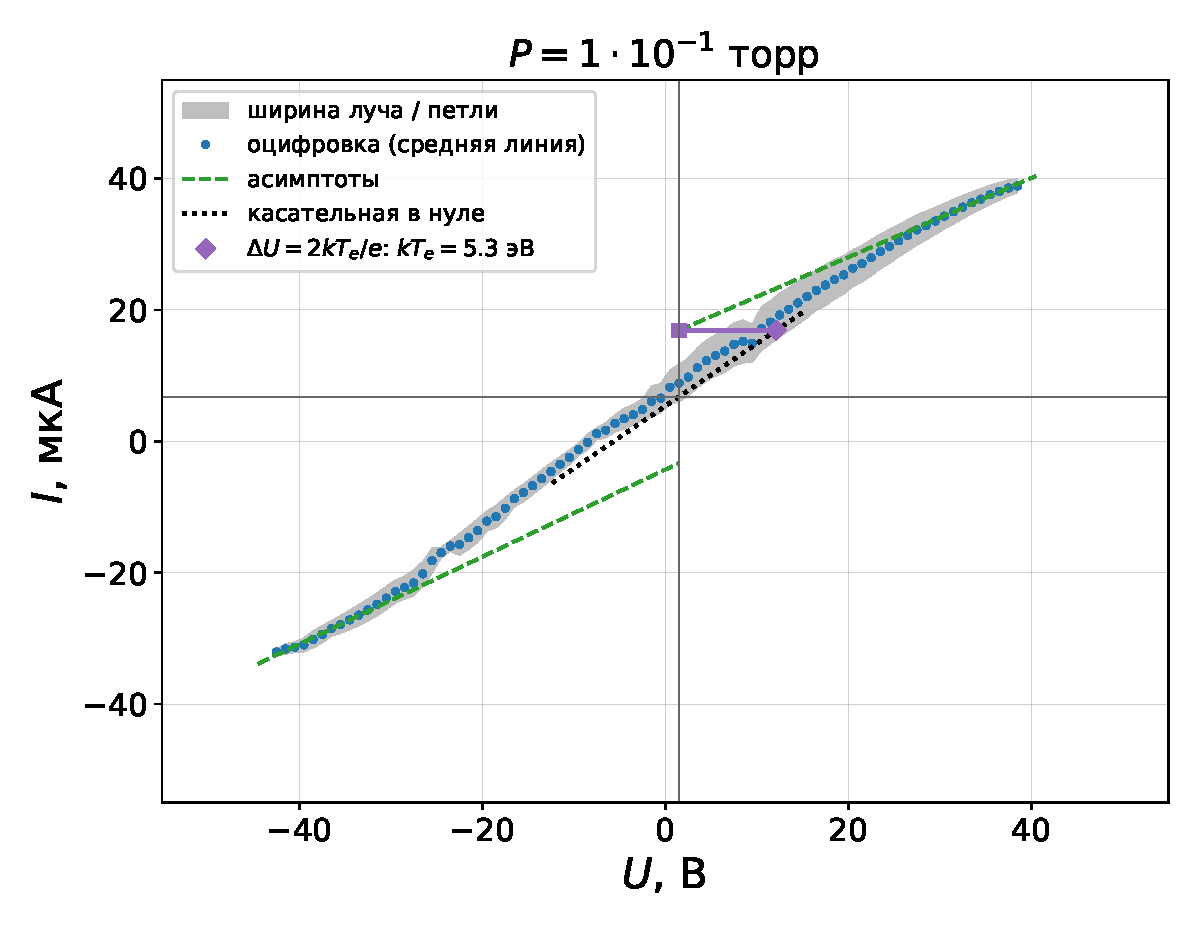
\includegraphics[width=0.8\linewidth]{vah_1e-1.pdf}
    \vspace{-1.5em} \caption{Вольт-амперная характеристика двойного зонда и определение её параметров при давлении $P = 0.10$~торр.}
    \label{fig:vah_1e1}
\end{figure*}

\begin{figure*}[t!]
    \centering
    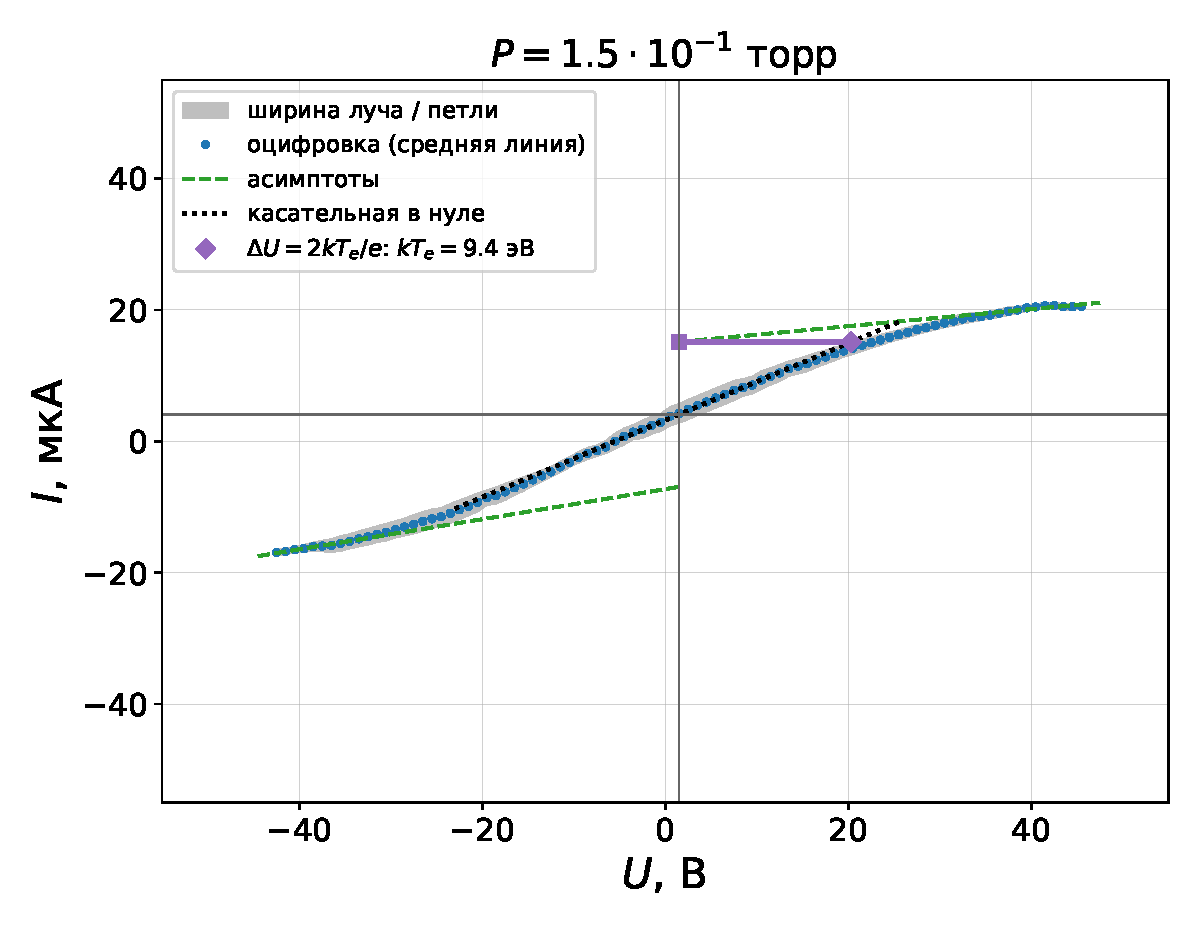
\includegraphics[width=0.8\linewidth]{vah_1.5e-1.pdf}
    \vspace{-1.5em} \caption{Вольт-амперная характеристика двойного зонда и определение её параметров при давлении $P = 0.15$~торр.}
    \label{fig:vah_15e1}
\end{figure*}

\begin{figure*}[t!]
    \centering
    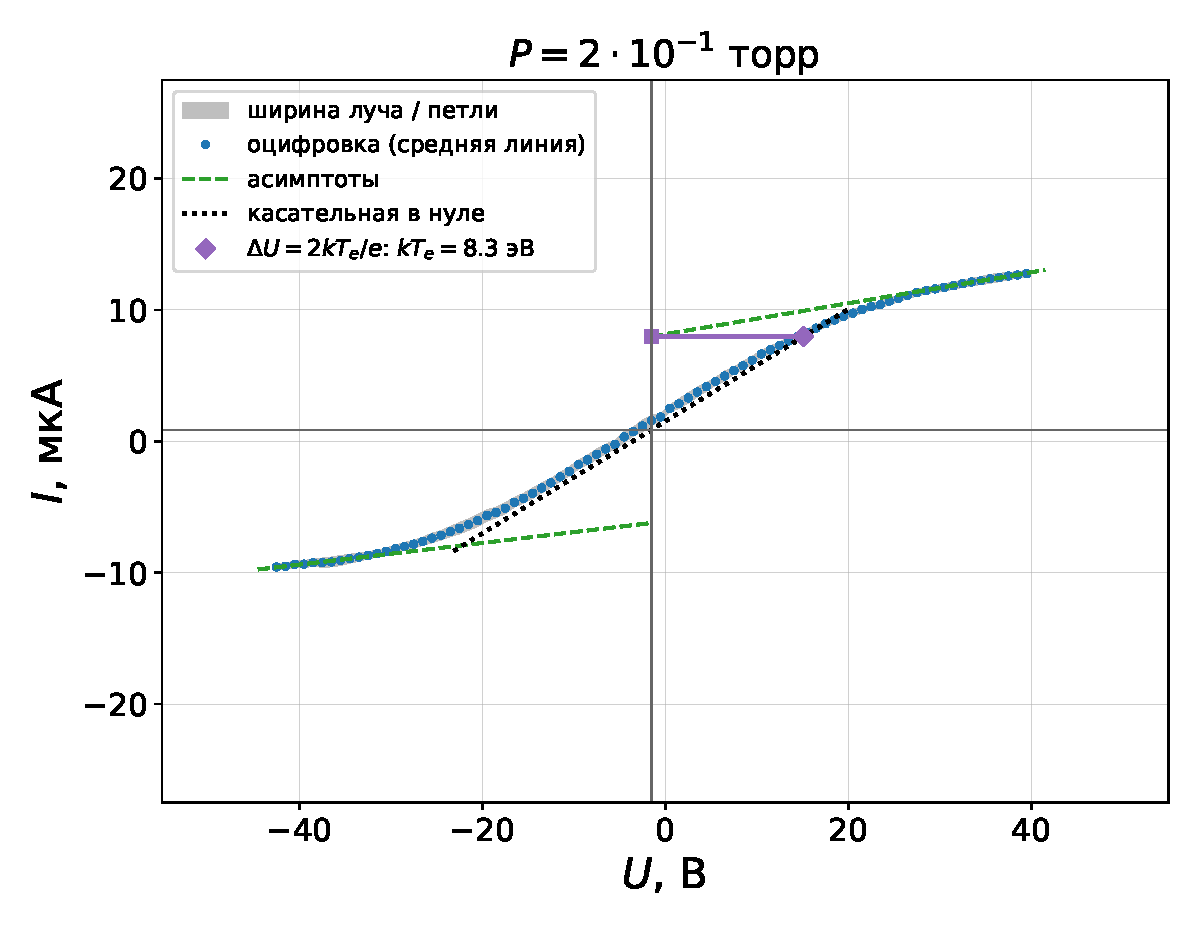
\includegraphics[width=0.8\linewidth]{vah_2e-1.pdf}
    \vspace{-1.5em} \caption{Вольт-амперная характеристика двойного зонда и определение её параметров при давлении $P = 0.20$~торр.}
    \label{fig:vah_2e1}
\end{figure*}



% --- Библиография ---
\begin{thebibliography}{99}

\bibitem{practicum2019}
Никулин М. Г., Попов П. В., Нозик А. А. и др. \textit{Лабораторный практикум по общей физике. В трёх томах. Т. 2. Электричество и магнетизм} / под ред. А. В. Максимычева, М. Г. Никулина. --- 2-е изд., перераб. и доп. --- М.: МФТИ, 2019. --- Раздел V, работа 3.5.2.

\bibitem{manual352}
\textit{Лабораторная работа 3.5.2 (4.16А) <<Исследование плазмы индукционного газового разряда>>. Дополнительное описание.} --- МФТИ, 2018.

\end{thebibliography}

\end{document}
